\documentclass[12pt, conference]{IEEEtran}
\IEEEoverridecommandlockouts
\usepackage{cite}
\usepackage{amsmath,amssymb,amsfonts}
\usepackage{algorithmic}
\usepackage{graphicx}
\usepackage{textcomp}
\usepackage{xcolor}
\usepackage[spanish]{babel}

\usepackage[%
    colorlinks=true,
    pdfborder={0 0 0},
    linkcolor=blue,
    citecolor=red
]{hyperref}

\renewcommand{\IEEEkeywordsname}{Palabras clave}

\def\BibTeX{{\rm B\kern-.05em{\sc i\kern-.025em b}\kern-.08em
    T\kern-.1667em\lower.7ex\hbox{E}\kern-.125emX}}
\begin{document}

\title{Survey introductorio a las definiciones, aplicaciones y métodos usados en el análisis de sentimientos\\
}

\author{\IEEEauthorblockN{
  Hansol Antay Rostrán}
\IEEEauthorblockA{\textit{Tecnológico de Costa Rica} \\
\textit{Escuela de Computación}\\
Limón, Costa Rica \\
rostrhan@outlook.com}
\and
\IEEEauthorblockN{Fredd Badilla Víquez}
\IEEEauthorblockA{\textit{Tecnológico de Costa Rica} \\
\textit{Escuela de Computación}\\
Limón, Costa Rica \\
frbadilla@estudiantec.cr}
\and
\IEEEauthorblockN{Randall Corella Castillo}
\IEEEauthorblockA{\textit{Tecnológico de Costa Rica} \\
\textit{Escuela de Computación}\\
Limón, Costa Rica  \\
randallcorella@estudiantec.cr}
}

\maketitle

\begin{abstract}
  En este survey se va a dar un repaso sobre el estado actual de los análisis de sentimientos en la era digital moderna. 
  Se denotarán conceptos básicos, técnicas, métodos, acercamientos, desafíos o limitaciones, junto con aplicaciones que se utilizan hoy en día. 
  Se analizarán desde modelos básicos para procesamiento de lenguaje natural, hasta modelos que utilizan aprendizaje automático. 
  La idea es brindar distintos aspectos que conllevan el análisis de sentimientos para compararlos y dar a conocer cómo es que se realizan estos procesos. 
  Se estudiarán las aplicaciones como el análisis de retroalimentación brindado por clientes de productos y servicios, el análisis de reputación de una empresa u organización, la predicción de movimientos sociales con potencial negativo, el estudio de la opinión pública sobre las campañas gubernamentales, el modelado de preferencias de usuario para anuncios, recomendaciones y demás. 
  Se pretende concluir este survey con un repaso de los conceptos más importantes, señalar los métodos y procedimientos para utilizados para el análisis de sentimientos, y el impacto que tiene este en la era digital tanto para las empresas como para los propios individuos.
\end{abstract}

\begin{IEEEkeywords}
component, formatting, style, styling, insert
\end{IEEEkeywords}

\section{Introducción}
El análisis de sentimientos es una disciplina que no es nueva, sino que se ha consolidado como una rama del procesamiento del lenguaje natural desde la década de 1950. 
En los últimos años, el análisis de sentimientos ha adquirido una gran importancia debido al auge de las redes sociales y la creciente disponibilidad de tecnologías para el procesamiento y modelado de la semántica del lenguaje. 
Para comprender su relevancia, es necesario plantearse cómo las plataformas digitales son capaces de recomendar canciones, vídeos o productos y cómo un simple tweet, comentario de Facebook o reseña en Amazon puede afectar significativamente a una empresa u organización. 
En este estudio, profundizaremos en los procesos utilizados por empresas u organizaciones en la toma de decisiones a partir de la comprensión de los conceptos básicos del análisis de sentimientos y el procesamiento del lenguaje natural.

En este trabajo, se explorarán diversos aspectos del análisis de sentimientos, desde los fundamentos computacionales hasta los aspectos psicológicos, y se describirán las técnicas y algoritmos utilizados por distintos procedimientos. 
Aunque se abordarán las limitaciones del análisis de sentimientos, como la detección de sarcasmo, ironía, negación o rechazo en el análisis textual, se evitará abordar temas ético-morales y de privacidad de los usuarios, ya que todos los métodos se basan en la recopilación masiva de datos públicos.

En una sección dedicada exclusivamente a los casos de uso, se presentarán ejemplos de aplicaciones del análisis de sentimientos en distintas industrias, enfocándose principalmente en la recopilación textual de texto, pero también mencionando otras aplicaciones que utilizan diferentes tecnologías. 
A través de estos casos prácticos, se ilustrarán los usos puntuales de dichos métodos en la vida cotidiana.

En la conclusión de este estudio, se repasarán las técnicas y aplicaciones del análisis de sentimientos que se han mencionado, comparado y estudiado. 
Se destacará la importancia e impacto que ha tenido el análisis de sentimientos en la industria, los hitos de las investigaciones mencionadas en todo el documento, la evolución de esta área en el ámbito computacional y empresarial, las limitaciones del campo de estudio y el alcance de futuras investigaciones relacionadas con el análisis de sentimientos.

\section{Conceptos y nociones fundamentales}
La presente sección es una reflexión sobre la definición de sentimientos, emociones y pensamiento, así como sobre la viabilidad del análisis de sentimientos desde una perspectiva computacional.

A pesar de que el enfoque principal sea computacional, todo va a girar en torno a los sentimientos, lo que lleva a la pregunta de cómo definir algo tan subjetivo. 
En este sentido, se debe hacer hincapié en que los sentimientos son el principal objeto de estudio y que para entenderlos es necesario conocer primero el ámbito psicológico y las emociones. 
Se define la emoción como un conjunto de reacciones psicológicas y fisiológicas generadas por el sistema límbico del cerebro y causadas por estímulos internos o externos que nos predisponen a reaccionar de cierta manera ante la situación. 
En cambio, los sentimientos son estados prolongados que se originan de la conceptualización racional de las emociones.

Una vez definidos estos conceptos, se plantea la cuestión de la viabilidad del análisis de sentimientos desde una perspectiva computacional. 
Se reconoce que el análisis de sentimientos es un problema abstracto, complejo y subjetivo, pero que, gracias a los avances tecnológicos, se han encontrado formas de captar, procesar e identificar las emociones y sentimientos expresados por los usuarios en diferentes plataformas. 

Detallaremos a continuación los conceptos básicos del análisis de sentimientos, es importante comprenderlos para poder adentrarnos más en casos de uso, aplicaciones y algoritmos o técnicas que son utilizadas en la actualidad. Todo esto con el fin de comparar y denotar los puntos fuertes y débiles de cada uno de ellos a medida que vamos presentando los casos de uso.

\subsection{Transfondo psicológico}
Tal como aplican en el estudio \cite{b1} del análisis de sentimientos en redes sociales, se debe tener en cuenta que este es un campo de estudio que se encuentra en constante evolución, por lo que es necesario tener en cuenta los avances que se han ido produciendo en el campo de la psicología. En dicho survey mencionan tres componentes principales de las emociones: la experiencia subjetiva, la respuesta fisiológica y la expresión conductual. Y su vez, lo diferencian del sentimiento, como la actitud mental que se desarrolla a partir de la experiencia emocional.

Incluso quitando un ámbito computacional al tema de análisis de sentimientos, \cite{b2} concluye que las emociones son una parte fundamental de la vida humana, ya que afectan nuestras decisiones y nos permiten comunicarnos mejor con el mundo. 
La detección de emociones implica identificar los diferentes sentimientos o emociones de una persona, pero detectar emociones a partir de texto es complicado debido a la gran cantidad de ambigüedades y jerga que se usan a diario. 
Además, la detección de emociones no se limita a identificar solo las condiciones psicológicas primarias (felicidad, tristeza, enojo), sino que puede llegar hasta 6 o 8 escalas según el modelo de emoción utilizado.

Como se mencionó anteriormente, pueden existir diferentes modelos de emoción, pero todos ellos se basan en la misma idea: identificar las emociones a partir de la expresión de un texto. Vamos a señalar dos categorías de modelos que servirán como ápice de muchas metodologías aplicadas en el análisis de sentimientos. En \cite{b3}, se menciona primero el modelo categórico de emociones. Este clasifica las emociones en categorías discretas y específicas, como la alegría, la tristeza, el miedo o la ira. Este modelo ha sido ampliamente utilizado en la psicología y en la investigación de las emociones.

Por otro lado, el modelo dimensional de emociones define las emociones como puntos en un espacio multidimensional, donde cada dimensión representa un aspecto emocional específico. Las dimensiones más comunes incluyen el valencia (positiva o negativa), la activación (alta o baja) y el control (alto o bajo).

A diferencia del modelo categórico, el modelo dimensional sugiere que las emociones no son mutuamente exclusivas y pueden existir en un continuo o espectro. Este modelo ha sido utilizado en la investigación de la neurociencia afectiva y en la psicología clínica para ayudar a comprender las emociones en un contexto más amplio.

\subsection{Limitaciones computacionales}
A pesar de los avances en el análisis de sentimientos desde una perspectiva computacional, todavía hay ciertas limitaciones en cuanto a la comprensión de los sentimientos y emociones expresados por los usuarios. 
Una de las limitaciones más importantes es la subjetividad inherente al análisis de sentimientos. 
Aunque los algoritmos pueden ser entrenados para reconocer ciertos patrones y palabras asociadas con emociones específicas, aún hay muchas expresiones que pueden ser interpretadas de diferentes maneras según el contexto o la cultura. 
Por lo tanto, el análisis de sentimientos no es una tarea fácil y requiere la implementación de técnicas avanzadas de procesamiento del lenguaje natural y aprendizaje automático.

Además, otro desafío importante es el procesamiento de grandes volúmenes de datos. 
El análisis de sentimientos implica el procesamiento de grandes cantidades de texto, lo que puede resultar en una sobrecarga de información. 
Los sistemas de análisis de sentimientos deben ser capaces de manejar grandes cantidades de datos de manera eficiente y efectiva, lo que requiere una gran cantidad de poder de procesamiento y almacenamiento de datos.

Otra limitación importante del análisis de sentimientos es la falta de contexto. 
A menudo, las expresiones de sentimientos se dan en un contexto específico, lo que puede afectar la forma en que se interpretan. 
Por lo tanto, la falta de contexto puede llevar a una interpretación errónea de los sentimientos expresados en un texto. 
Para superar esta limitación, se han desarrollado técnicas avanzadas que utilizan el contexto para comprender mejor el significado de las expresiones de sentimientos. Además, el análisis de sentimientos también puede ser limitado por la calidad y cantidad de los datos disponibles. 
Para entrenar a los algoritmos de análisis de sentimientos, se necesitan grandes cantidades de datos de alta calidad. 
Si los datos utilizados para el entrenamiento son incompletos o no representan la realidad, los algoritmos de análisis de sentimientos pueden no ser precisos. 
Por lo tanto, es importante asegurarse de que los datos utilizados para el entrenamiento sean precisos y representativos.

A pesar de que se han realizado grandes avances en el análisis de sentimientos desde una perspectiva computacional, todavía hay varias limitaciones que deben ser superadas. 
La subjetividad inherente al análisis de sentimientos, la falta de contexto, la sobrecarga de información, la calidad y cantidad de los datos disponibles son algunas de las limitaciones más importantes que deben ser abordadas para lograr una mayor precisión en el análisis de sentimientos.

Uno de los puntos que vamos a resaltar en este survey es referente a como poder detectar sarcasmo e ironía en un texto. El trabajo de investigación \cite{b4} es todo un estudio sobre como el sarcasmo es un gran desafío para los modelos de análisis de sentimientos, ya que puede ocultar la intención real de desprecio y negatividad detrás de una representación positiva. La detección de sarcasmo es importante para comprender los verdaderos sentimientos y creencias de las personas. El sarcasmo es difícil de identificar tanto para humanos como para máquinas debido a su figuratividad y sutileza. La detección automática de sarcasmo se ha abordado como un problema de clasificación binaria y se ha centrado principalmente en recursos léxicos y pragmáticos, así como en cambios sentimentales en las oraciones. Sin embargo, el sarcasmo a menudo se manifiesta de manera implícita, lo que dificulta la identificación para las máquinas.

\subsection{Fina brecha del aprendizaje automático}
Para adentrarnos más adelante en métodos y algoritmos sofisticados que se utilizan en el análisis de sentimientos aprovecharemos la cuestión de si es necesario o no aplicar aprendizaje automático para el análisis de sentimientos. 
En \cite{b5} denotan muchos conceptos y elementos utilizados en el análisis de sentimientos. Esto nos brindará una excusa para hablar de la fina brecha que existe entre el aprendizaje automático y el análisis de sentimientos, mientras introducimos conceptos e ideas base detras de los algoritmos y métodos que se utilizan.

\subsubsection{Análisis sin aprendizaje automático}
La idea más básica que se puede dar del análisis de sentimientos es que es una recopilación de palabras y frases que se utilizan para expresar sentimientos positivos o negativos. Por lo que se puede decir que el análisis de sentimientos es una tarea de clasificación de texto. Para ello no es requerido el aprendizaje automático, se puede realizar tomando en cuenta los siguientes elementos:
\begin{itemize}
\item \textbf{Cuantificación de palabras}: El conteo, la frecuencia y la ponderación de las palabras se utilizan para cuantificar el sentimiento de un texto. Este simplemente se basa en una idea muy sencilla: \textit{contar las palabras positivas y negativas en un texto, para luego determinar si el texto es positivo o negativo}.
\item \textbf{Heurísticas}: El concepto de heurística en el ámbito de procesamiento de texto lo vamos a definir como ciertas reglas que se utilizan para determinar el sentimiento de un texto compuesto. 
A diferencia de la cuantificación de palabras, las heurísticas no se basan en el conteo de palabras, sino en el análisis de la estructura del texto. 
Por ejemplo, si un texto comienza con una palabra negativa, entonces el texto es negativo.
\item \textbf{Diccionarios de sentimientos}: Los diccionarios de sentimientos son una colección de palabras y frases que se utilizan para expresar sentimientos positivos o negativos. 
Estos diccionarios se utilizan para determinar el sentimiento de un texto. 
Por ejemplo, si un texto contiene palabras positivas, entonces el texto es positivo. 
A diferencia de las heurísticas, los diccionarios de sentimientos no se basan en la estructura del texto, sino en el contenido del texto.
\item \textbf{Bolsa de palabras}: Es una representación textual que describe la aparición de palabras en un documento. Se registra el recuento de palabras, ignorando los detalles gramaticales y el orden de las palabras. Se llama "bolsa de palabras" porque se descarta cualquier información sobre el orden o la estructura de las palabras en el documento. Este es un método muy utilizado en el área de NLP.
\end{itemize}

\subsubsection{Análisis con aprendizaje automático}
Vamos a definir el aprendizaje automático como un conjunto de técnicas que permiten a las computadoras aprender de los datos sin ser explícitamente programadas. En este apartado vamos a mencionar elementos que nos ayudarán a entender el aprendizaje automático y su relación con el análisis de sentimientos.

\begin{itemize}
\item \textbf{Aprendizaje supervisado}: El aprendizaje supervisado es un tipo de aprendizaje automático en el que se entrena un modelo utilizando datos etiquetados. Haciendo uso de este tipo de aprendizaje, se puede entrenar un modelo para predecir el sentimiento de un texto.
\item \textbf{Representación textual}: Parte del aprendizaje supervisado es la representación textual, y va más allá de la cuantificación de palabras y las heurísticas. Depende mucho del modelo que se utilice, pero en general, la representación textual se basa en la idea de que las palabras que aparecen en un texto tienen un significado.
\item \textbf{Selección de características}: La selección de características es un paso importante en el aprendizaje supervisado. Veremos más adelante como podemos hacer uso de bolsas de palabras, n-gramas y otros elementos para seleccionar características.
\item \textbf{Hiperparametrización}: La hiperparametrización es un proceso que se utiliza para optimizar los parámetros de un modelo. Estos sirven para ajustar el modelo a los datos de entrenamiento, de manera que el modelo pueda generalizar mejor nuevos datos. Algunos hiperparámetros son: el número de capas, el número de neuronas por capa, la función de activación, el optimizador, profundidad del árbol de decisión, el número de épocas, etc.
\item \textbf{Validación cruzada}: La validación cruzada es un método de evaluación de modelos que se utiliza para evaluar la precisión de un modelo. El proceso de validación es muy sencillo, se divide el conjunto de datos en k partes, se entrena el modelo k veces, cada vez utilizando una parte diferente como conjunto de prueba y el resto como conjunto de entrenamiento. Al final se promedian los resultados de las k pruebas para obtener un resultado final.
\end{itemize}

Ya con una vez comprendidos estos elementos básicos, deberíamos tener una visión más clara sobre como funcionan procesos complejos de análisis de sentimientos, como el aprendizaje automático. De forma intuitiva, podríamos darnos una idea de como funcionan internamente la mayoría de modelos planteados para el análisis de sentimientos.

En la continuación de la sección, veremos términos más puntuales y técnicos que serán referenciados cuando expliquemos y comparemos los diferentes métodos y algoritmos que se utilizan en el análisis de sentimientos.

\subsection{Procesamiento de Lenguaje Natural}

El procesamiento de lenguaje natural (PLN) es una rama de la inteligencia artificial que se encarga de estudiar y desarrollar métodos para que las computadoras puedan procesar lenguaje natural. 
El procesamiento de lenguaje natural es un campo muy amplio, y se puede dividir en varias áreas, como la comprensión del lenguaje natural, la generación de lenguaje natural, la traducción automática, la extracción de información, la clasificación de texto, etc. 
En esta sección vamos a centrarnos en la clasificación de texto, que es una de las áreas más importantes del procesamiento de lenguaje natural que va de la mano con el análisis de sentimientos.

En el mismo sentido, el PLN tiene como objetivo fundamental extraer el significado o la semántica del lenguaje. 
La semántica es el estudio de las palabras y su relación con el mundo real, se refiere la capacidad que se tiene de entender el significado de una oración o un texto. 
No solamente es analizar las palabras y estructuras gramaticales, sino también, de darles un sentido. 
Esto se hace a través de diversas técnicas y algoritmos, en su mayoría basados en el aprendizaje automático y el procesamiento de cantidades masivas de información. 
Todo esto para analizar y extraer patrones, significados y relaciones entre palabras y textos. 
Todo esto permitiendo a las computadoras entender el lenguaje humano, mediante la toma de decisiones de forma autónoma.

En \cite{b6} se menciona el surgimiento del PLN estadístico, este enfoque se basa en la idea de que el lenguaje natural sigue ciertas regularidades estadísticas que se pueden modelar con precisión utilizando técnicas de estadística y aprendizaje automático. 
Por ejemplo, se pueden utilizar modelos probabilísticos para predecir la probabilidad de que una palabra aparezca en un contexto determinado o para determinar la relación semántica entre palabras. 
En \cite{b7} se da una breve introducción al PLN estadístico, y en \cite{b8} se mencionan algunos de los algoritmos más utilizados en el PLN estadístico, además de problemas comunes de este enfoque. Estas investigaciones son importantes que ya nos permite clasificar las tareas de PLN en dos grandes grupos: las tareas de bajo nivel y las tareas de alto nivel.

\subsubsection{Tareas de bajo nivel}
\begin{itemize}
  \item \textbf{Detección de límites de oraciones}: también conocida como (SBD) por sus siglas en inglés, Sentence Boundary Detection, es la tarea de identificar los límites de las oraciones en un texto.
  Es una tarea importante, sobretodo en áreas como la traducción automática, la generación de texto, la extracción de información, el análisis de sentimientos, etc. Para ello se pueden hacer de métodos basados en reglas, modelos probabilísticos y aprendizaje automático.
  Puede llegar a hacer un proceso muy complejo, ya que las oraciones pueden llegar a ser muy complejas, contener muchas cláusulas o frases, lo que puede ser difícil determinar donde termina una oración y empieza otra.
  Sin mencionar que en un texto pueden haber abreviaturas, acrónimos, citaciones u otros signos de puntuación que pueden llegar a confundir a los modelos.
  \item \textbf{Tokenización}: esta tarea consiste en dividir un texto en unidades más pequeñas, llamadas tokens. Pueden ser palabras, símbolos, números, o incluso una frase completa.
  Este es un paso fundamental para el análisis de sentimientos, ya que es necesario dividir el texto en palabras para poder analizar cada una de ellas por separado. En \cite{b9} se mencionan algunas utilizadas para la tokenización de textos, tales como la tokenización por espacios, la tokenización por expresiones regulares, la tokenización por palabras, la tokenización por frases, etc.
  Los métodos más utilizados son: la tokenización por espacios, que es la más sencilla ya que consiste en dividir el texto en tokens por espacios; la tokenización por signos de puntuales, que puede llegar a ser eficiente para texto formal, pero no para texto coloquial; la tokenización por análisis morfológico, que consiste en analizar la estructura morfológica de las palabras para dividirlas en tokens, permitiendo una tokenización muy precisa.
  \item \textbf{Decomposición morfológica}: este implica en dividir la palabra en componentes morfológicos, como la raíz, el sufijo, el prefijo, y demás. Esta parte proporciona información útil sobre el significado y la estructura de una palabra.
  \item \textbf{Part-of-speech tagging}: también conocido como POS tagging, es la tarea de asignar una etiqueta a cada palabra en un texto, indicando su categoría gramatical. Por ejemplo, si la palabra es un sustantivo, un verbo, un adjetivo, etc.
  \item \textbf{Shallow parsing}: también conocido como análisis sintáctico superficial, es la tarea de identificar las relaciones sintácticas entre las palabras de un texto. Por ejemplo, si una palabra es el sujeto de una oración, el objeto directo, el objeto indirecto, etc. Hace uso de etiquetas gramaticales identificadas en el POS tagging. En \cite{b10} y \cite{b11} se mencionan como se preparan los datos, y concluyen que independientemente del modelo empleado para el análisis de texto, lo que en realidad influye más al momento de analizar resultados es la cantidad de datos de entrenamiento y la calidad de los mismos.
\end{itemize}

\subsubsection{Tareas de alto nivel}
Propiamente, las tareas de bajo nivel son más generalizadas. Por otro lado, las tareas de alto nivel son trabajadas en base a las tareas de bajo nivel, y suelen ser más específicas. En \cite{b12} presentan un modelo incremental para el manejo de múltiples tareas de PLN, con una profundidad creciente. Entre algunas tareas de alto nivel se encuentran:
\begin{itemize}
  \item \textbf{Identificación de errores gramaticales y ortográficos}: este tipos de tareas pueden ser muy volátiles, se puede dar el caso de detectar falsos positivos (errores que no existen) o falsos negativos (errores que no se detectan).  En \cite{b13} \cite{b14} exponen modelos basados en la estructuración y análisis de texto mediante el uso de redes neuronales recurrentes, comparandolos con modelos tradicionales.
  \item \textbf{Named Entity Recognition}: también conocido como NER, es la tarea de identificar entidades nombradas en un texto. Por ejemplo, si una palabra es un nombre propio, un lugar, una fecha, etc. En \cite{b15} desarrollan un modelo basado en redes neuronales para aprender relaciones complejas en grandes cantidad de texto. En \cite{b16} y \cite{b17} exploran técnicas mediante usos de aprendizaje supervisado y no supervisado, sistemas NERC y aprendizaje automático basado en reglas.
\end{itemize}
Se profundizarán estas y otras tareas a continuación, lo dejaremos de momento como ejemplos de como se pueden clasificar las tareas de PLN.

\subsubsection{Named Entity Recognition}\label{subsubsec:NER}
Aprovecharemos en listar algunos retos al momento de realizar NER, para generalizar conceptos que se pueden aplicar en el ámbito del procesamiento de texto de forma general, algunos de estos retos son: 
\begin{itemize}
  \item \textbf{Variación del orden de palabras o frases}: esto se da cuando una entidad nombrada se encuentra en una posición diferente en el texto, pero se refiere a la misma entidad.
  \item \textbf{Derivación}: esto permite que varias palabras se refieran a la misma entidad, más comúnmente denominado como la raíz de la palabra. Varias derivaciones de una misma raíz pueden tener diferentes significados, por ejemplo, las palabras "comer", "comeedor" y "come" pueden verse como diferentes derivaciones de una misma raíz "com" y que se puedan clasificar de esa misma forma.
  La derivación puede se tiene que entender desde un ámbito léxico, en lugar de un ámbito semántico.
  \item \textbf{Homógrafos}: esto se da cuando dos o más palabras se escriben de la misma forma, pero tienen significados diferentes. Por ejemplo, la palabra "banco" puede referirse a un banco de un río, o a un banco de una institución financiera. Esto puede confundir a muchos modelos de NER, ya que no pueden distinguir entre ambas palabras. Para ello se requieren de otros métodos para poder identificar la entidad nombrada, métodos enfocados en un ámbito semántico y no léxico. En \cite{b18} se propone un método de desambiguación de homógrafos no supervisado que se basa en técnicas de agrupamiento y asignación semántica. Concluyendo mediante resultados experimentales que es un método eficiente en comparación a otros métodos no supervisados.
\end{itemize}

\subsubsection{Frecuencia y cercanía de palabras}

La frecuencia y cercanía de palabras va muy de la mano con el procesamiento de lenguaje natural. La frecuencia de palabras se refiere a la cantidad determinada de veces que aparece una palabra en un determinado texto. 
Debido a que mucho métodos hacen uso de técnicas probabilísticas este valor se suele representar como un porcentaje. 
Mientras que la cercanía de palabras se hace referencia a que tan cerca se suelen encontrar unas palabras de otras. 
Ambos parámetros son de gran importancia en el ámbito computacional, por un lado, la frecuencia nos ayuda a determinar la importancia de una determinada palabra o frase en un texto en particular y la cercanía de palabras nos va a ayudar a la identificación de patrones usuales o relaciones que pueden tener unas palabras con otras.

\subsection{Modelado espacio-temporal de datos}\label{subsec:Modelado}

Uno de los retos más importantes para el análisis y procesamiento de texto es que no siempre vamos a tener la información en un formato estructurado, por ejemplo, en un archivo de texto plano.
Al trabajar con cantidades masivas de datos, y a su vez, con texto coloquial como el que se encuentra en las redes sociales, es muy común que la información obtenida no sea muy fácil de procesar. 
En \cite{b19} se propone comprender patrones de comportamiento en redes sociales mediante el análisis de texto. Se busca analizar la tendencia de los usuarios en las redes sociales, para buscar que palabras son más utilizadas en ciertas regiones geográficas, o en ciertos momentos.
La definición para estudiar y analizar los momentos puede variar un montón, por ejemplo, se puede analizar el comportamiento en un día, en una época del año o en un periodo de tiempo determinado.

Este tipo de análisis puede ayudar a la predicción de eventos, como por ejemplo, la predicción de la cantidad de personas que asistirán a un evento, o la predicción de la cantidad de personas que se infectarán de una enfermedad en un determinado periodo de tiempo.
Este enfoque en particular es muy importante, el análisis de patrones espaciales y temporales en redes sociales son muy útiles en el área de la sociolingüística, la economía, e incluso la política.

\subsection{Modelos basados en aspectos}

En esta sección no vamos a profundizar técnicas utilizadas en el análisis de sentimientos basado en aspectos. Lo que es importante denotar en este acercamiento es que el enfoque en aspectos nos permite a identificar y analizar sentimientos que fueron expresados en un texto que son específicos de un determinado producto, servicio, entidad u organización.
En \cite{b21} se describe la importancia de estos modelos en la industira y desafíos que presenta. Posteriormente en este survey vamos a detallar los métodos o acercamientos más utilizados en estos modelos. Los conceptos más importantes a denotar son:

\begin{itemize}
  \item \textbf{Clasificación de polaridad}: este proceso permite determinar si un determinado aspecto es positivo, negativo o neutro. Asignando un valor numérico a cada aspecto que es analizado.
  \item \textbf{Generación de resúmenes de sentimiento}: este es más un componente que implica la síntesis de sentimientos que fueron expresados en un determinado texto. Permite a usuarios tener una visión general de los sentimientos expresados sobre un determinado producto, servicio, entidad u organización. Este aspecto será muy importante para entender como este tipo de modelos influyen en la toma de decisiones.
  \item \textbf{Stopwords}: son palabras que se encuentran en un determinado texto que no aportan información relevante. Por ejemplo, las palabras "la", "los", "las", etc.
\end{itemize}

\subsection{Medición de calidad de modelos de lenguaje}

La medición de calidad de modelos de lenguaje es un aspecto muy importante en el área de procesamiento de lenguaje natural. Hasta este punto hemos comprendido como podemos hacer uso de modelos de lenguajes para realizar procesos como el análisis sentimientos. Además de definir algunos conceptos que son importantes para entender el funcionamiento de estos modelos. Si bien el diseño, implementación y entrenamiento de estos modelos es un proceso muy complejo y muy variado en cuanto a los algoritmos que se utilizan, la medición de calidad de estos modelos es un aspecto que se suele pasar por alto.
Haremos mención de algunos métodos para evaluar la calidad de los modelos de lenguaje, pero no profundizaremos en ellos, este apartado servirá cuando hagamos mención a estos métodos en el resto del survey (sobretodo cuando hagamos comparaciones entre modelos). En \cite{b22, b23, b24, b25, b26} se detallan varios de estos, algunos de los métodos más utilizados son:
\begin{itemize}
  \item \textbf{Perplexity}: es medida permite indicar la capacidad de un modelo de lenguaje para predecir la siguiente palabra en una secuencia de palabras. Se calcula como la inversa de la probabilidad de la secuencia de palabras. Cuanto menor sea el valor de la perplexity o perplejidad, mejor será el modelo y que tan bueno es ajustándose a los datos de entrenamiento.
  \item \textbf{Precisión, exhaustividad y F1-score}: estos valores son muy utilizados para medir la calidad de los modelos de clasificación. Se calculan a partir de la matriz de confusión. La precisión es la proporción de predicciones positivas que son correctas.
  \[\frac{verdaderosPositivos}{verdaderosPositivos + falsosPositivos}\]
  La exhaustividad es la proporción de verdaderos positivos que fueron identificados correctamente.
  \[\frac{verdaderosPositivos}{verdaderosPositivos + falsosNegativos}\]
  El F1-score es la media armónica entre la precisión y la exhaustividad. De forma más precisa:
  \[\frac{2 * precision * exhaustividad}{precision + exhaustividad}\]
  \item \textbf{A/B Testing}: este método permite comparar dos modelos de lenguaje. Se utiliza para determinar si un modelo es mejor que otro. Se utiliza para comparar modelos de lenguaje en diferentes dominios, por ejemplo, comparar un modelo de lenguaje para el dominio de la salud con un modelo de lenguaje para el dominio de la política. También se puede utilizar para evaluar y comparar dos versiones de un mismo modelo de lenguaje. En este método se consideran muy importantes las métricas de tiempo de respuesta o la tasa de error.
\end{itemize}

\subsection{Unigramas, bigramas y n-gramas}

Estos son términos utilizados para referirse a las distintas combinaciones de palabras que se pueden utilizar para entrenar un modelo de lenguaje. Por ejemplo, unigramas son palabras individuales, bigramas son dos palabras que se encuentran juntas, y n-gramas son n palabras que se encuentran juntas. En la siguiente imagen se puede observar un ejemplo de unigramas, bigramas y n-gramas.

\begin{table}[h]
\centering
\begin{tabular}{|c|c|c|}
\hline
\textbf{Unigramas} & \textbf{Bigramas} & \textbf{Trigramas} \\ \hline
\textit{El} & \textit{El perro} & \textit{El perro es} \\ \hline
\textit{perro} & \textit{perro es} & \textit{perro es un} \\ \hline
\textit{es} & \textit{es un} & \textit{es un animal} \\ \hline
\textit{un} & \textit{un animal} & \textit{} \\ \hline
\textit{animal} & \textit{} & \textit{} \\ \hline
\end{tabular}
\caption{Unigramas, bigramas y n-gramas}
\label{tab:my_label}
\end{table}

\subsection{Corpus}

En palabras resumidas, en análisis de sentimientos un corpus es un conjunto de documentos o textos que se utilizan como una base para entrenar y probar distintos modelos de análisis de sentimientos. Este se puede crear con diversas fuentes permitiendo a investigadores y analistas entrenar sus modelos enfocados en el aprendizaje automático. La mayoría de veces (más adelante veremos que no necesariamente) el corpus es etiquetado de forma manual con sentimientos positivos, negativos o neutros. Lo más importante a la hora de definir un corpus es que sea lo más representativo posible del dominio que se quiere analizar. Por ejemplo, si se quiere analizar sentimientos en el dominio de la salud, el corpus debe estar compuesto por textos relacionados con la salud.

\section{Casos de uso o ejemplos}

En esta sección se presentan algunos ejemplos de casos de uso de modelos de lenguaje. Estos ejemplos se presentan para mostrar como estos modelos pueden ser utilizados en diferentes áreas.

\begin{itemize}
  
% Ejemplo:
\item En el paper \cite{r1} hacen una presentación de una nueva tecnica denominada Análisis de Sentimiento de Documentos Online "SAOOP". 
Puede evaluar los comentarios de sentimiento en línea en el ámbito de los artículos de investigación.
Esta técnica es una que introduce una mejora del modelo Bag-of-Words para las
principales debilidades del modelo de bolsa de palabras en la evaluación.
\item En el artículo \cite{r2}  utilizan los n-gramas para el enfoque basado en caracteres, un rasgo que demostró ser significativo
en los trabajos de Reyes et al., (2013) and Ptácek et al., (2014).
\item En el artículo \cite{r3} se hace mención a la idea Bos (Bag of synsets) la cual se aplica
a estudios de investigación relacionados con la minería de textos en otros idiomas también. Sin embargo, en los
últimos años, la atención de la investigación a este modelo ha disminuido bajo el efecto del modelo Bolsa de
Conceptos (BoC).
\item En el artículo \cite{r4} se menciona la utilización de Naïve Bayes y fuzzy clustering para el
análisis del sarcasmo en microblogs en Twitter.
\item En el artículo \cite{r5} se referencia (BoWK) la bolsa de palabras de kernel y como este concepto 
crea relaciones semánticas entre tweets mediante vectores.
\item En el artículo \cite{r6} mencionan el (LSK) léxico semántico de kernel y como la información
 léxica de los tweets puede ser muy escasa, para ampliar el modelo BoW, proporcionaremos
 otra representación vectorial
 para generalizar la información léxica. Puede obtenerse para cada término de un diccionario mediante un
 espacio de palabras de co-ocurrencia construido según el Análisis Distribucional descrito en (Sahlgren, 2006)
 Se construye una matriz palabra por contexto, M, mediante el análisis de corpus a gran escala y, a continuación, se procesa mediante
 Análisis Semántico Latente (Landauer y Dumais, 1997).
 \item En el artículo \cite{r7} se menciona la existencia del (USPC) contexto del perfil de sentimiento
 del usuario, que se puede utilizar como referencia para predecir los sentimientos del usuario.
 \item En el paper \cite{r8}  se describe que las técnicas orientadas al léxico para la
 de la polaridad del sentimiento se basan en 
 diferentes léxicos, como WordNet y
 SentiWordNet (SWN) [10, 11,12]. Para la detección de sentimientos a partir de comentarios del usuario en YouTube.
 \item En el survey \cite{r9} se utiliza la técnica de clasificación Naïve Bayes para el análisis de sentimientos. El clasificador se entrena en la
 base de datos IMDb (basado en el análisis realizado en el
 investigación). El conjunto de entrenamiento consta de 5000 críticas de películas positivas y
 5000 críticas de películas negativas respectivamente. Los comentarios
 para cada palabra clave se utilizan como datos de prueba para la clasificación.
 clasificación. El tamaño de los datos de prueba varía para cada palabra clave y oscila entre un mínimo de 10.000 (datos de Dow Jones) y un máximo de 300.000 (Obama).
 hasta 300.000 (Obama). El clasificador Naïve Bayes se entrena con los comentarios del conjunto
 para calcular el sentimiento general de cada comentario del
 de prueba.
 \item En \cite{r19} se hace un enfoque en la investigación de la opinión de los usuarios en línea. Más específicamente, para la predicción de compras de productos haciendo uso de análisis de datos de series temporales en redes sociales.
 \item \cite{r18} argumenta sobre los modelos tradicionales que se han utilizado hasta el momento para investigar la comunicación política en Twitter. Los modelos tradicionales se han enfocado en masivas cantidades de datos, lo que puede llevar a una falta de comprensión de los procesos en la plataforma, en su lugar, se propone un estudio de subconjuntos más pequeños que permitan obtener más a detalle el análisis realizado a la comunición de ámbito político realizado en la plataforma. Se propone de esta forma debido a que hay patrones de comunicación que se pueden perder en grandes conjuntos de datos por lo que en un contexto electoral, un acercamiento más preciso permite una compresión más detallada de la o las estrategias y tácticas políticas utilizadas por candidatos y partidos políticos.
 \item En \cite{r17} de igual forma hace uso de datos de Twitter para intentar predecir movimientos en el mercado de valores. En la investigación se correlacionaron el análisis de polaridad de sentimientos a tweets que estaban ligados de alguna forma a la bolsa de valores. Sin embargo, en dicho estudio solo se hace sugerencia que dicha polaridad era acertiva para intentar predecir cambios en los valores del mercado. Dicha herramienta se concluyó como una herramienta útil para predecir movimientos en el mercado de valores, pero que se requiere de un análisis muy cuidadoso para poder llegar a conclusiones más sólidas.
 \item En \cite{r16} se realizó un estudio de datos recopilados de Twitter durante un período de dos semanas en abril de 2020. Los tweets fueron recolectados utilizando palabras clave relacionadas con COVID-19 y se utilizaron técnicas de preprocesamiento de texto para limpiar los datos y eliminar los tweets irrelevantes. Se utilizaron técnicas de detección de temas y análisis de sentimientos para analizar los tweets. La detección de temas se realizó utilizando un modelo de tema latente (LDA), que identificó los temas más comunes en los tweets. El análisis de sentimientos se realizó utilizando un modelo de clasificación de sentimientos (SVM), que clasificó cada tweet como positivo, negativo o neutral. Los resultados del estudio mostraron que los temas más comunes en los tweets relacionados con COVID-19 en Brasil eran la política y la salud, mientras que en Estados Unidos eran la economía y la salud. Además, los tweets relacionados con la política tenían sentimientos más negativos en ambos países, mientras que los tweets relacionados con la salud tenían sentimientos más positivos. Este tipo de estudio puede ayudar a los gobiernos a comprender mejor la opinión pública sobre COVID-19 y a tomar decisiones más informadas.
 \item En \cite{r15} se pretende llevar el análisis de sentimientos en un entorno médico, entre estos se menciona la identificación de síntomas, evaluación de la eficacia de algún tratamiento en particular y una forma más precisa de documentar de forma analítica la experiencia del paciente. Lamentablemente el estudio realizado menciona varias limitaciones que impiden y/o dificultan el uso del análisis de sentimientos en un entorno médico, entre estas se menciona la falta de datos previamente etiquetados y el problema de interpretación subjetiva de datos. Adicionalmente, se menciona que debido a las políticas sobre la privacidad de datos médicos representan un desafío muy importante, ya que los datos de salud son muy sensibles y deben protegerse de forma adecuada.
 \item \cite{r14} se centra en la aplicación de análisis de sentimientos para detectar actividades fraudulentas de dinero en plataformas de comercio electrónico. El objetivo del estudio es desarrollar un método temprano de detección de actividades fraudulentas de dinero mediante el análisis de los sentimientos en los comentarios de los compradores. El estudio utiliza una combinación de análisis de sentimientos y técnicas de aprendizaje automático para detectar patrones en los comentarios de los compradores que puedan indicar actividades fraudulentas de dinero. Se recopilaron datos de comentarios de compradores de dos sitios web de comercio electrónico populares, y se utilizó un modelo de clasificación de sentimientos para identificar patrones en los comentarios que indicaran actividades fraudulentas.
 \item En \cite{f4} se estudia un enfoque semiautomático o híbrido para la anotación de emociones en textos de redes sociales. Dicha propuesta es llamada EmoLabel, está fundamentanda en técnicas de aprendizaje automático y en la intervención humana para el etiquetado de los textos con las emociones correspondientes. La idea básica de este método es tener un conjunto de datos previamente etiquetados de forma manual, luego se utilizan técnicas de aprendizaje automático para la creación de modelos que permitan clasificar emociones a textos que no se encuentren clasificados de ninguna forma. Dicho proceso se repite varias veces con el objetivo de ir entrenando al modelo agregando de forma gradual más textos etiquetados de forma manual hasta alcanzar cierto nivel de precisión o satisfacción según los parámetros predefinidos por análistas y diseñadores del modelo. La parte de la intervención humana se utiliza para verificar y corregir las etiquetas que se han generado de forma automático por el modelo, aumentando de esta forma la precisión del criterio de clasificación de emociones. Lo más importante a destacar de este método es que se trabajan con datos recopilados de redes sociales, en donde no se suelen tener datos necesariamente formales y estructurados, pero de igual forma mantiene un alto nivel de precisión en la clasificación de emociones. Se menciona también que dicho enfoque se escalable y adaptable a diferentes idiomas y a otros tipos de textos. Cabe destacar la investigación \cite{f5} en donde se sigue un enfoque similar pero utilizando exclusivamente datos de Twitter.
 \item En \cite{f6} se presenta un estudio bastante interesante, en donde se utiliza un enfoque autónomo para etiquetar las emociones en diarios de sueños haciendo uso de técnicas de procesamiento de lenguaje natural. Primero se recopilan los diarios de sueño de un grupo de participantes voluntarios y se les pidió que anotaran las emociones que experimentaron durante sus sueños. Luego, se utilizó un modelo de NLP entrenado en un corpus de texto emocional para etiquetar automáticamente las emociones en los diarios de sueños. El estudio evaluó la precisión del modelo de NLP y comparó sus resultados con las anotaciones manuales de las emociones en los diarios de sueños. Los resultados mostraron que el modelo de NLP fue capaz de etiquetar correctamente las emociones en los diarios de sueños en un alto porcentaje de casos. Dicho estudio se señaló importante en las áreas de psicología enfocadas a la salud mental y la detección de transfornos o patrones no saludables del sueño en las personas.
 \item En \cite{f7} se menciona aplicaciones del análisis semántico latente, permite analizar grandes cantidades de texto mediante descomposiciónde valores singurales. Este paper describe varias aplicaciones de este acercamiento para la clasificación de documentos e incluso la detección de plagio. Veremos más adelante como se utiliza este método en el análisis de sentimientos de forma más detallada. Siguiendo la misma línea, \cite{f10} también menciona el análisis indexado latente, en donde se usan n-gramas para visualizar la autoría de documentos. De igual forma vamos a detallar más adelante como se utiliza este método en el análisis de sentimientos.
 \item En \cite{f11} veremos como se describe el desarrollo de un sistema de monitoreo para detectar posibles usuarios que presenten indicios de depresión haciendo uso del análisis de sentimientos. Este sistema se va a basar en una recopilación de texto enviados por usuarios a través de plataformas de distintas redes sociales y aplicaciones de mensajería. Estos mensajes son procesados para evaluar el detalle emocional de los mismos. Este sistema hace uso de un modelo de aprendizaje automático para la identificación de patrones de lenguaje asociados con la depresión, y en caso de que el sistema detecte una posible señal de depresión se envía una notificación al usuario recomendando ayuda profesional.

\end{itemize}

\section{Algoritmos o técnicas utilizadas}
En esta sección veremos un poco más en detalle algoritmos o técnicas que fueron o no mencionados a lo largo del survey. Utilizaremos el diagrama de la ``Figura~\ref{fig3}'' para enfocarnos y señalar los métodos de análisis de sentimientos que se han utilizado en los papers revisados de una forma más apropiada. Se recopiló gran parte de la información de la investigación de \cite{f2}, además de la información de los papers revisados.

\begin{figure}[htbp]
  \caption{Repaso de métodos utilizados para el análisis de sentimientos.}
  \centerline{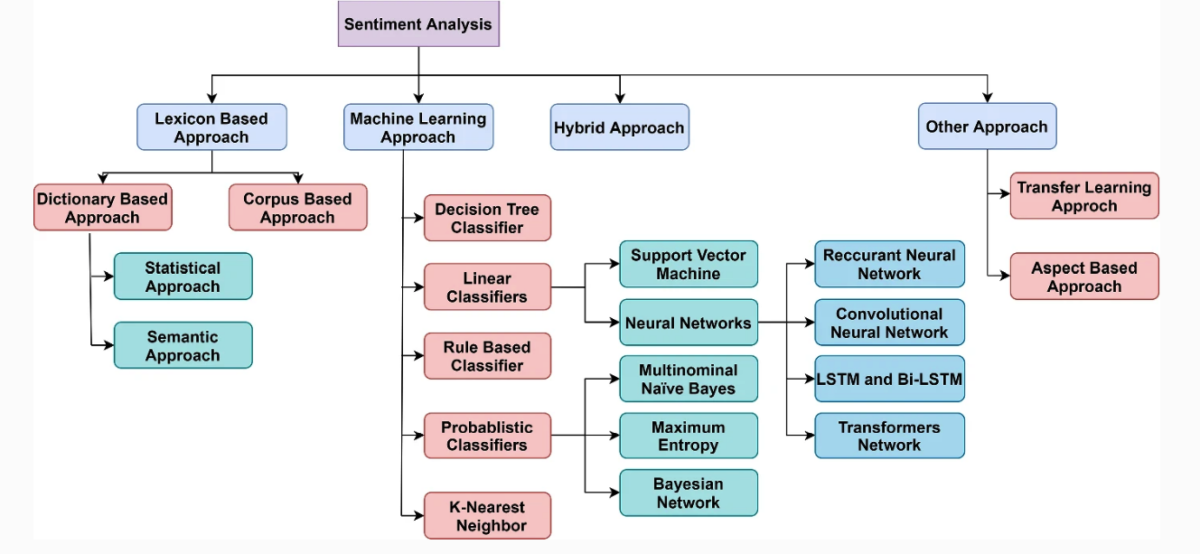
\includegraphics[width=0.51\textwidth]{IMG´s/tecnicas_analisis_sentimientos.png}}
  \label{fig3}
\end{figure}

\subsection{Enfoque basado en léxico}
Estos métodos simplemente están basados en el uso de diccionarios de palabras con algunas notaciones de polaridad para clasificar la opinión en un texto determinado. La premisa es simple, pero se pueden dar distintos enfoques al momento de elegir las características o parámetros para el análisis de sentimientos. En \cite{f7} hace un estudio sobre distintos diccionarios de palabras con polaridad y distintos métodos de clasificación de polaridad de las palabras. Como el método de contar palabras, el método de análisis semántico latente y el método de análisis de componentes principales.
\begin{itemize}
  \item \textbf{Método de análisis semántico latente}: referido también como \textit{latent semantic analysis} (LSA), es un método que se basa en la descomposición de valores singulares de una matriz de términos que va por documentos, cada término es representado como una columna y cada documento está representado por una fila. El trabajo de descomposición permite reducir el tamaño de la matriz y extraer los conceptos latentes que subyacen entre los términos y los documentos. En la ``Figura~\ref{fig5}'' podemos ver una representación visual de ejemplo de dicha matriz.
  \begin{figure}[htbp]
    \caption{Matriz de términos usados en LSA}
    \centerline{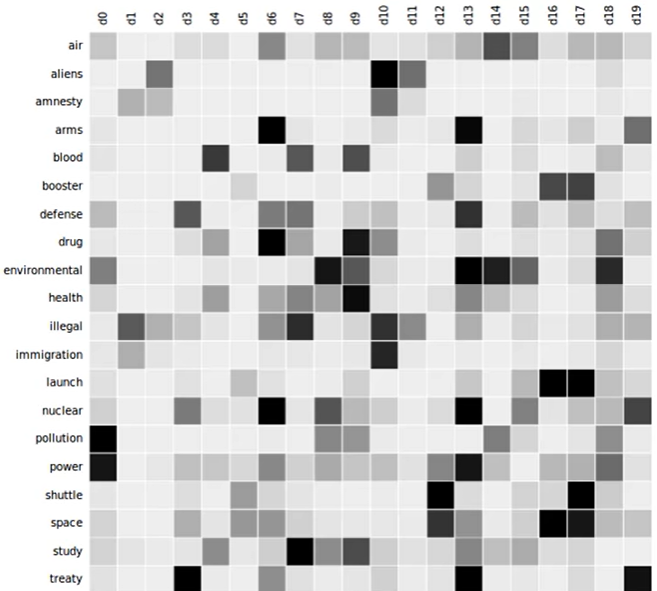
\includegraphics[width=0.51\textwidth]{IMG´s/matriz LSA.png}}
    \label{fig5}
  \end{figure}
  La descomposición permite que dichos conceptos puedan ser representados mediantes vectores, los cuales pueden ser usados para representar los documentos y los términos. En la ``Figura~\ref{fig6}'' podemos ver un ejemplo de cómo se representan los documentos y los términos en un espacio vectorial.
  \begin{figure}[htbp]
    \caption{Representación vectorial en LSA }
    \centerline{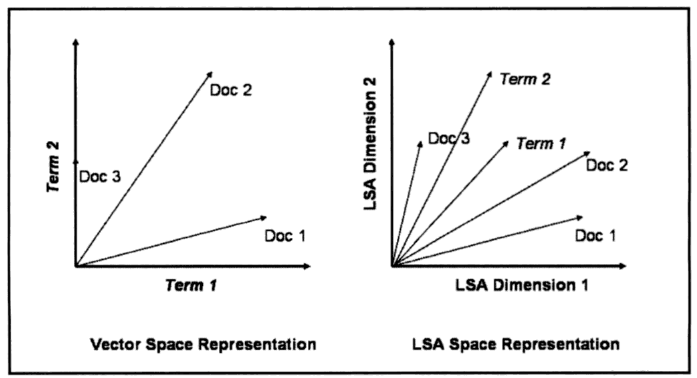
\includegraphics[width=0.51\textwidth]{IMG´s/vectores LSA.png}}
    \label{fig6}
  \end{figure}
  En \cite{f9} se explica más a detalle como este método reduce la dimensionalidad de los datos para fácil representación.

  \item \textbf{Método de análisis semántico-indexado latente}: esta variante se utiliza de igual formas para analizar un gran volumen de documentos, mayormente usados para la detección de plagio y identificación de autores que no sean tan conocidos. En \cite{f10} proponen una técnica que combina el análisis de frecuencia de los n-gramas en los documentos con el análisis de conceptos latentes para visualizar la autoría de los documentos. La premisa de este acercamiento se basa en la idea de que los autores tienen un estilo de escritura único que se puede detectar mediante el análisis de los n-gramas utilizados en sus textos. Además, los autores proponen el uso de LSI para analizar los conceptos latentes que subyacen a los documentos, lo que permite una representación más compacta de la información y una comparación más fácil entre los documentos. Más que todo se enfocan en dar una representación visual del estilo de escritura de algunos autores, y además, que se pueda diferenciar y detectar distintos patrones de escritura entre los documentos. En la investigación citada anteriormente se usan dos autores, Daniel y el Rey Salomón, para demostrar la efectividad de la técnica propuesta. Más específicamente, se utilizan dos textos que son atribuidos al Rey Salomón: \textit{Song of Songs} y \textit{Ecclesiastes}, y textos en general que no son específicados que son atribuido a Daniel. Es importante a destacar que los textos elegidos del Rey Salomón son distintos entre sí, el contenido textual y semántico varía entre ambos textos, ya que uno es un poema y el otro es un libro de filosofía, pero ambos son atribuidos al Rey Salomón. En la ``Figura~\ref{fig7}~\ref{fig8}~\ref{fig9}'' podemos ver gráficamente como los textos de Daniel y el Rey Salomón se diferencian entre sí, y como los textos del Rey Salomón presentan una mayor similitud entre sí.
  \begin{figure}[htbp]
    \caption{Primeras dos dimensiones escalonadas del SVD.}
    \centerline{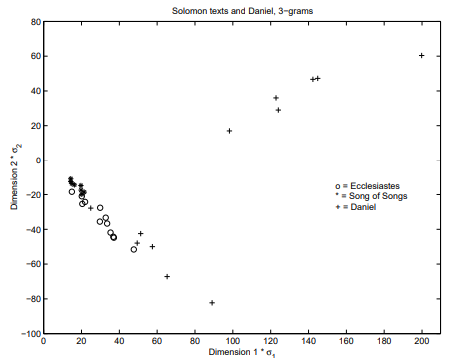
\includegraphics[width=0.51\textwidth]{IMG´s/tabla1 LSI - Salomon.png}}
    \label{fig7}
  \end{figure}
  \begin{figure}[htbp]
    \caption{Valores de la primera dimensión de cada libro.}
    \centerline{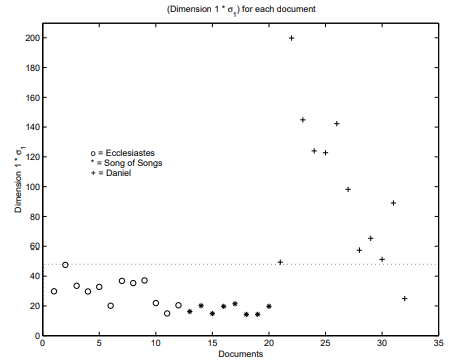
\includegraphics[width=0.51\textwidth]{IMG´s/tabla2 LSI - Salomon.png}}
    \label{fig8}
  \end{figure}
  \begin{figure}[htbp]
    \caption{Valores de la segunda dimensión de cada libro.}
    \centerline{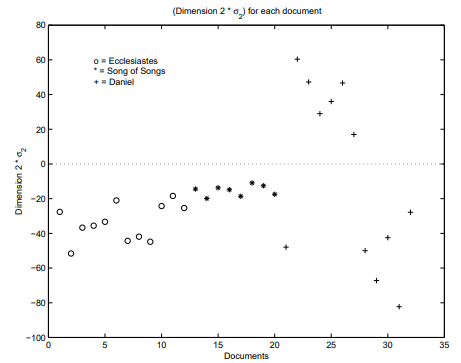
\includegraphics[width=0.51\textwidth]{IMG´s/tabla3 LSI - Salomon.png}}
    \label{fig9}
  \end{figure}
\end{itemize}

\subsection{Métodos basados en diccionarios}
Estos métodos son bastantes sencillos y se han hecho mención de ellos en todo el survey. Estos son bastante útiles para la extracción específica de texto, clasificación de texto o análisis de sentimientos. Def forma general se puede explicar este métodos son los siguientes pasos:

\begin{itemize}
  \item \textbf{Creación del diccionario}: se crea un diccionario que contenga palabras o frases relevantes para el dominio central de interés. Ya sea de forma manual o de forma automatizada.
  \item \textbf{Se identifican palabras o frases clave}: se busca en el texto todas esas palabras o frases que fueron marcadas con anterioridad. Se puede detectar haciendo uso de un criterio exacto o basado en similitudes.
  \item \textbf{Extracción de información relevante}: una vez se identifican las palabras o frases clave, se usa dicha información para analizar o clasificar el texto según convenga.
\end{itemize}

\subsection{Métodos basados en corpus}

Los métodos basados en corpus son útiles para grandes procesamientos de textos. La idea base es parecida con el acercamiento basado en diccionarios, la diferencia es que en estos métodos se pretende detectar patrones y estructuras del lenguaje natural.

\begin{itemize}
  \item \textbf{Preparación del corpus}: se recopila la información suficiente para formar el corpus de datos y se prepara el análisis para eliminar palabras irrelevantes al contexto o ámbito.
  \item \textbf{Extracción de características}: se detectan características del corpus, como por ejemplo la frecuencia de palabras, co-ocurrencia de palabras, patrones o similutudes semánticas o léxicas y demás.
  \item \textbf{Entrenamiento del modelo}: se entrena el modelo con el corpus de datos y se obtiene un modelo que puede ser usado para clasificar o analizar textos.
  \item \textbf{Evaluación del modelo}: se evalúa el modelo con un conjunto de datos de prueba para determinar la efectividad del modelo.
\end {itemize}

\subsection{Métodos basados en aprendizaje automático}

Estos métodos residen en un enfoque en inteligencia artificial para el desarrollo y mejora de modelos de aprendizaje automático. Estos métodos se basan en el uso de algoritmos de aprendizaje automático para la detección de patrones y estructuras en los textos. Estos métodos se pueden clasificar en dos grandes grupos: supervisados y no supervisados.

\subsubsection{Árboles de decisión}

Los árboles de decisión utilizan una serie de características para tomar decisiones sobre la polaridad de algún texto en específico. Estos árboles son construidos a partir de un conjunto de datos de entrenaimentos para representar polaridades emocionales. La construcción de estos árboles implica la selección de una característica en cada nodo del árbol, que ayudan a tomar decisiones más específicas sobre la polaridad del texto. Se puede construir mediante la idea de entropía, que es una medida de la incertidumbre de un sistema. La entropía se puede calcular de la siguiente forma:

\begin{equation}
  H(X) = -\sum_{i=1}^{n} p(x_i) \log_2 p(x_i)
\end{equation}
Además, a medida que se va descendiendo en el árbol se pueden afinar más los parámetros de la polaridad del texto. En la Figura \ref{fig10} se muestra un ejemplo de un árbol de decisión para la detección de polaridad emocional.
\begin{figure}
  \centering
  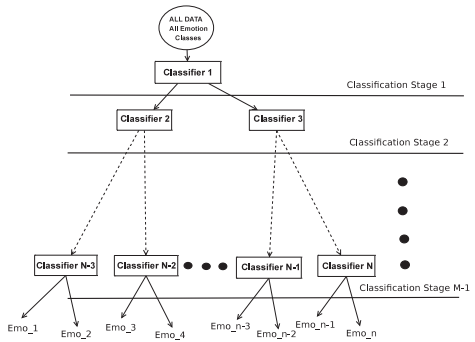
\includegraphics[width=0.5\textwidth]{IMG´s/arbol de decision 01.png}
  \caption{Ejemplo de un árbol de decisión para la detección de polaridad emocional.}
  \label{fig10}
\end{figure}

Lo más importante a destacar, es que en los niveles más bajos del árbol se suelen considerar los casos con mayor ambiguedad, que se suelen clarificar mediante del análisis del camino tomado en el árbol ya que dichos datos son los que más incertidumbre generan. En \cite{f14} más a detalle esta estructura y se comparan los resultados con otros métodos.


\subsubsection{Clasificadores lineales}

Los clasificadores lineales son métodos de aprendizaje supervisado que se basan en la idea de clasificar un texto en una categoría o clase. Estos métodos se basan en la idea de que los datos se pueden separar mediante una línea o hiperplano. Más propiamente, en el análisis de sentimientos se pueden utilizar varias características como la frecuencia de palabras, el tono de palabras, longitud de la oración, entre otras. Una vez identificada las características se procede a entrenar el modelo lineal. Existen varios tipos de clasificadores lineales pero denotaremos dos muy utilizados en el análisis de sentmientos:
\begin{itemize}
  \item \textbf{Regresión logística}: es un clasificador lineal que se basa en la idea de que las características de un texto pueden ser representadas por un vector de características. En este caso se hace uso de una función logística para calcular la probabilidad de que un texto sea positivo o negativo:
  \begin{equation}
    P(y=1|x) = \frac{1}{1 + e^{-w^Tx}}
  \end{equation}
  En donde los parámetros $w$ son los pesos de las características y $x$ es el vector de características. La función logística se puede ver en la Figura \ref{fig15}.
  \begin{figure}
    \centering
    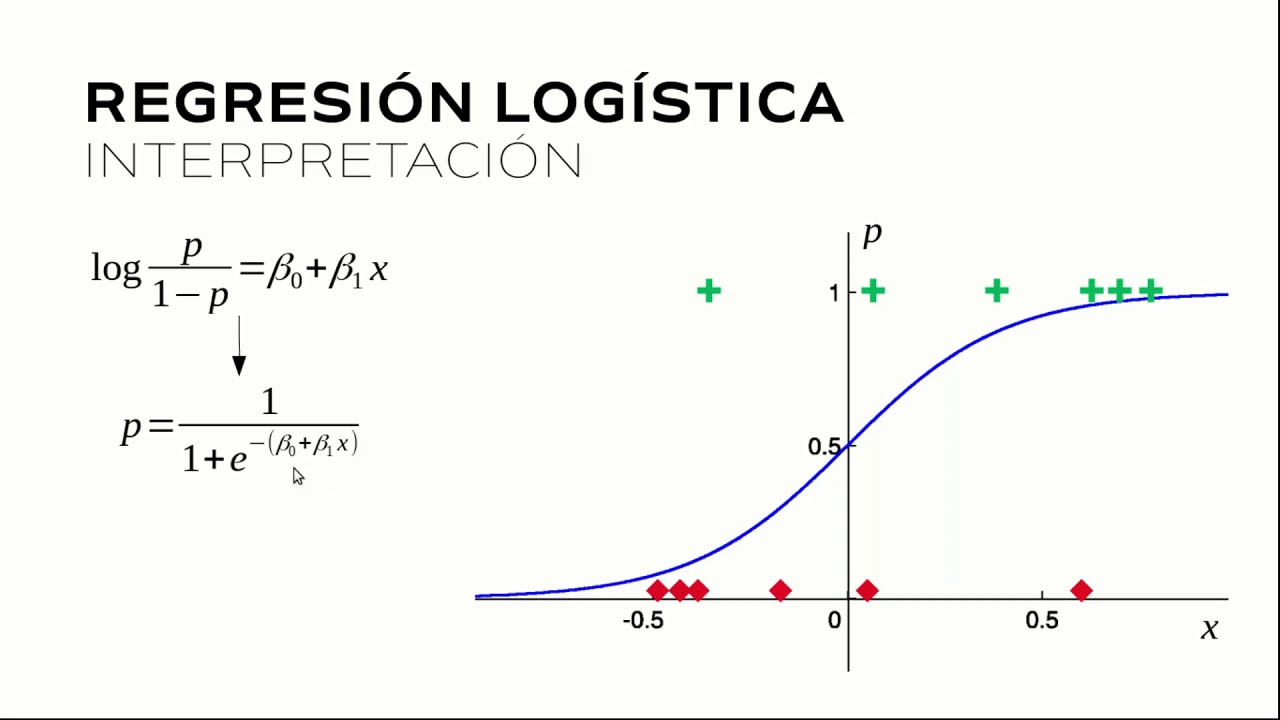
\includegraphics[width=0.5\textwidth]{IMG´s/regresion logistica.jpg}
    \caption{Función de regresión logística.}
    \label{fig15}
  \end{figure}
  Lo más importante a destacar es que la función logística es una función sigmoide que se puede utilizar para clasificar un texto en una categoría o clase.
  \item \textbf{Máquinas de vectores de soporte}: este es un algoritmo de aprendizaje automático para la clasificación de datos. El objetivo primordial es encontrar un hiperplano en un espacio de características que separe los datos de diferentes clases de una forma óptima. Los textos que se encuentran en un lado del hiperplano se clasifican como positivos y los que se encuentran en el otro lado se clasifican como negativos. Si bien hay muchas similitudes entre la regresión logística y las máquinas de vectores de soporte, la diferencia más importante es que la regresión logística se basa en la idea de que los datos se pueden separar mediante una línea o hiperplano, mientras que las máquinas de vectores de soporte se basan en la idea de que los datos se pueden separar mediante un margen. En la Figura \ref{fig16} se muestra un ejemplo de una máquina de vectores de soporte.
  \begin{figure}
    \centering
    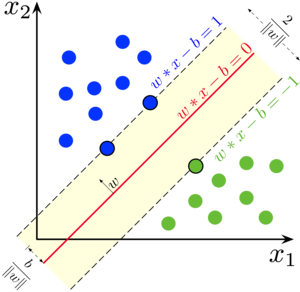
\includegraphics[width=0.4\textwidth]{IMG´s/mvs.png}
    \caption{Máquinas de vectores de soporte.}
    \label{fig16}
  \end{figure}

  \item \textbf{Long Short-Term Memory}: este es un tipo específico de red neuronal recurrent utilizado para el análisis de sentimientos. La variante que ofrece el LSTM es que tiene una memoria a largo plazo, lo que le permite aprender patrones en secuencias de datos de larga duración. Este método utiliza celdas que están conectadas a través de puertas que controlan la entrada, la salida y la actualización de la información. En la Figura \ref{fig17} se muestra un ejemplo de una celda LSTM.
  \begin{figure}
    \centering
    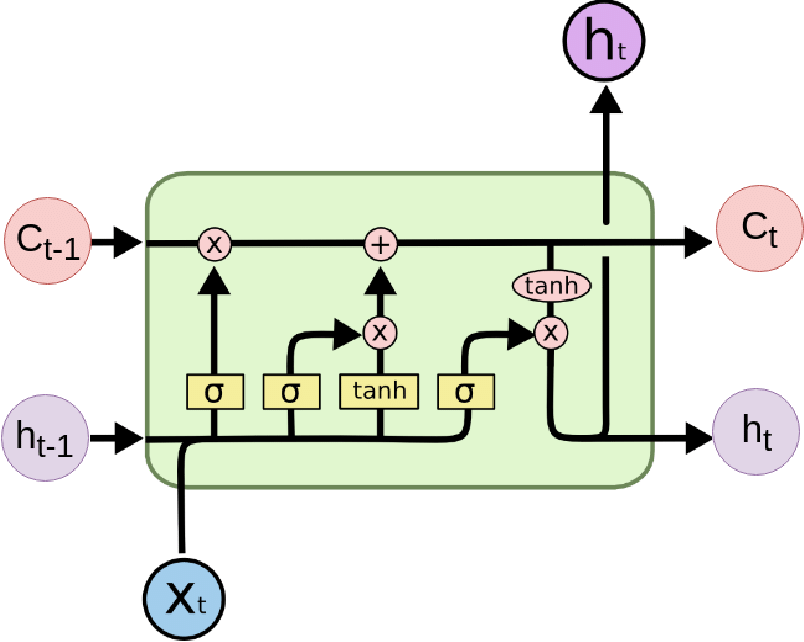
\includegraphics[width=0.4\textwidth]{IMG´s/celda rnn lstm.png}
    \caption{Celda LSTM.}
    \label{fig17}
  \end{figure}

  \item \textbf{Identificadores basados en reglas}: son una técnica de clasificación en el aprendizaje automático que se basa en un conjunto de reglas explícitas para tomar decisiones sobre la clase de una instancia de entrada. Son básicamente un montón de reglas if-then que se utilizan para procesar la lógica interna al momento de deliberar el significado de un texto. 
  \item \textbf{Clasificadores bayesianos}: utilizan un modelo probabilístico que estima la probabilidad de que una instancia pertenezca a cada clase en función de las características o atributos de la instancia. Luego, se utiliza el teorema de Bayes para calcular la probabilidad posterior de que la instancia pertenezca a cada clase, utilizando la probabilidad previa y la probabilidad de los atributos. Primero que nada recordando el teorema de Bayes:
  \begin{equation}
    P(A|B) = \frac{P(B|A)P(A)}{P(B)}
  \end{equation}
  Estos clasificadores pueden ser de dos tipos: \textit{Naive Bayes} y \textit{Bayesian Network}. En el caso del \textit{Naive Bayes} se asume que las características son independientes entre sí, mientras que en el caso de \textit{Bayesian Network} se asume que las características no son independientes entre sí. En la Figura \ref{fig18} se muestra la idea intuitiva de una red bayesiana.
  \begin{figure}
    \centering
    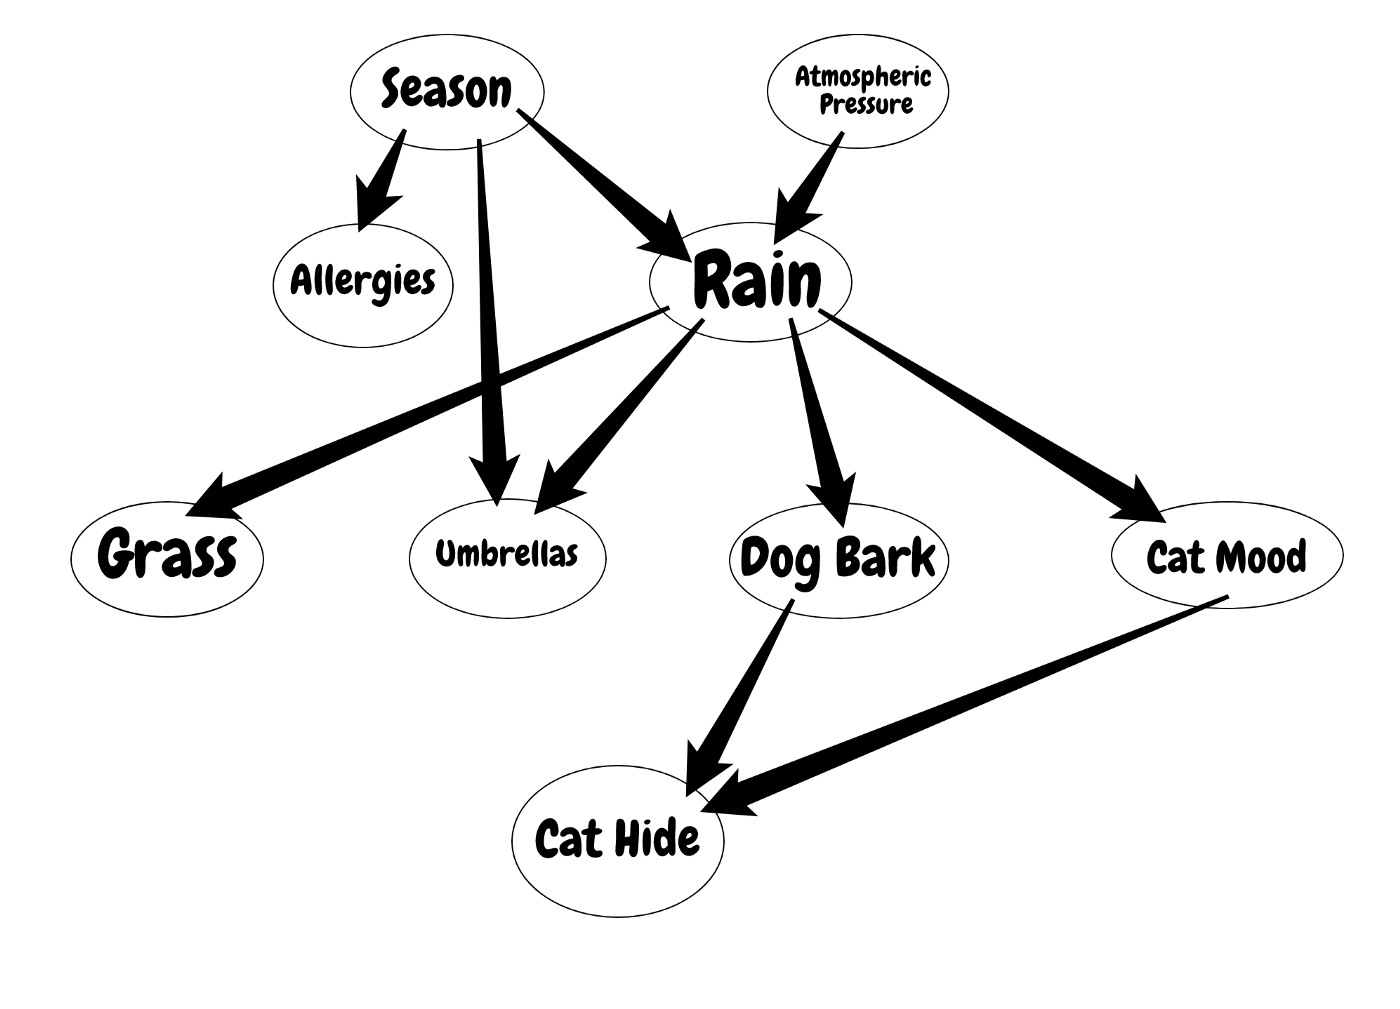
\includegraphics[width=0.4\textwidth]{IMG´s/bayesian network.png}
    \caption{Idea intuitiva de una red bayesiana.}
    \label{fig18}
  \end{figure}

  \item \textbf{k-NN}: es un algoritmo de aprendizaje automático que se utiliza para clasificación y regresión. El objetivo de este algoritmo es encontrar los k vecinos más cercanos de una instancia de entrada y luego asignarle la clase que más se repite entre los vecinos. En la Figura \ref{fig19} se muestra un ejemplo de k-NN.
  \begin{figure}
    \centering
    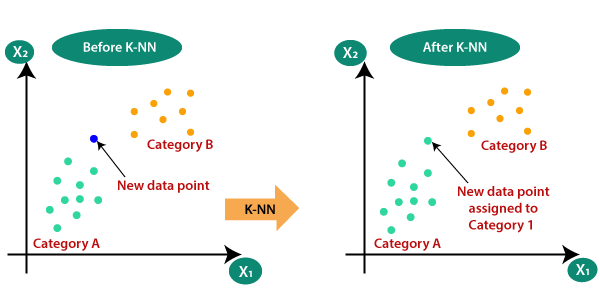
\includegraphics[width=0.4\textwidth]{IMG´s/knn.png}
    \caption{Gráfica del proceso k-NN.}
    \label{fig19}
  \end{figure}
\end{itemize}

\subsection{Anotación de emociones}
De forma generalizada, la anotación de emociones es una forma en la que se puede clasificar un texto mediante etiquetas que indiquen la emoción expresada ya sea por palabras o por oraciones. Esto se puede aplicar de forma manual o de forma automática. En \cite{f3} se describe un estudio para diseñar técnicas de anotación emocional en tiempo real para videos de realidad virtual. El objetivo del estudio es mejorar la experiencia del usuario y la inmersión en los videos de VR, al permitir una retroalimentación de la experiencia emocional del usuario en tiempo real. En dicha investigación se hace énfasis en dos técnicas: modelo de botón de respuesta continua y la otra, un modelo de deslizador de respuesta continua, en donde ambas formas requieren una interacción directa del usuario, pero que ofrece una retroalimentación instantánea y precisa de la experiencia emocional del usuario. A continuación veremos ejemplos similares en donde vamos a comparar y señalar distintos acercamientos que se han investigado hasta la fecha para la anotación de emociones. En el paper se hace mención de cuestiones éticas sobre el uso de información personal pero nos enfocaremos más en la idea propuesta por la investigación, además de técnicas para encriptación de datos personales.
%%%%%%%%%%%%%%%%%%%%%%%%%%%%%%%%%%%%%%%%%%%%%%%%%%%%%%%%%%%%%%%%

\subsection{Perfilado emocional}
Más que un método se puede considerar un concepto, pero es algo que se puede utilizar de forma amplia en el campo del análisis de sentimientos. El perfilado de personas se refiere al proceso de generar "perfiles" de usuarios mediante datos pasados que estén relacionados a un usuario en particular. En \cite{f12} se explica como se utilizan datos personales de usuario para adaptar recomendaciones en motores de búsqueda. Dicho sistema se basa en tener partes de un mismo perfil distribuido de distintas formas en donde asocian uno o más dispositivos para el monitoreo de las actividades y preferencias del usuario para luego registrar todo en un servidor de forma que se pueda analizar y predecir las emociones del usuario. La arquitectura se puede visualizar mejor en la ``Figura~\ref{fig10}''.
\begin{figure}[htbp]
  \caption{Arquitectura propuesta para perfilado emocional.}
  \centerline{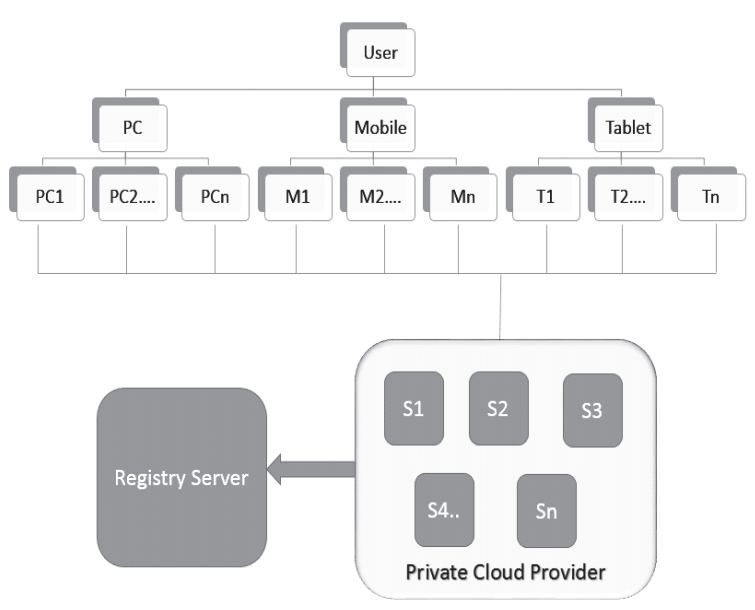
\includegraphics[width=0.4\textwidth]{IMG´s/arquitectura de perfil de usuario.png}}
  \label{fig10}
\end{figure}

\subsection{Reconocimiento facial}
Se utiliza para hacer captura de las expresiones provenientes de los locutores, ya que estás dicen mucho sobre una situación, se tuvo ciertas complicaciones, sobre todo cuando una persona cambiaba de emoción drásticamente, haciendo que al ERC se le complicara determinar el estado de la persona, por esto se implementó un historial de emociones, donde se ira almacenando las expresiones de la persona, para así determinar la razón del cambio de expresión. En \cite{f13} se mencionan una gran cantidad de métodos y algoritmos pero podemos rescatar los siguientes como los más destacables:

\begin{itemize}
  \item \textbf{Redes neuronales convolucionales}: este tipo de redes naurales son comúnes en el análisis de imágenes. Tienen la capacidad de extraer características de forma automática y es por ello que se consideran muy importante en el paper. En este tipo de redes neuronales se tienen distintas capas, entre ellas las capas convolucionales, las cuales se encargan de extraer características de la imagen, como por ejemplo, bordes, texturas, etc. En la ``Figura~\ref{fig11}'' se puede ver un ejemplo de una capa convolucional.
  \begin{figure}[htbp]
    \caption{Ejemplo de una capa convolucional.}
    \centerline{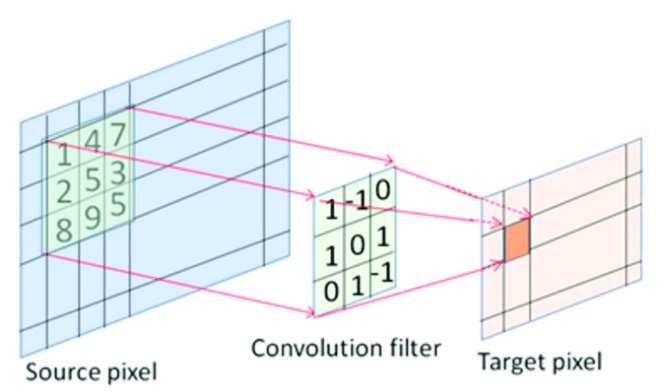
\includegraphics[width=0.4\textwidth]{IMG´s/filtro convolucional CNN.png}}
    \label{fig11}
  \end{figure}
  \item \textbf{Histogramas de orientación de gradientes (HOG)}: este método se basa en la detección de bordes, es decir, se busca la dirección de los bordes de la imagen, para así poder determinar la orientación de la cara. En la ``Figura~\ref{fig12}'' se puede ver un ejemplo de un histograma de orientación de gradientes.
  \begin{figure}
    \caption{Ejemplo de un histograma de orientación de gradientes.}
    \centerline{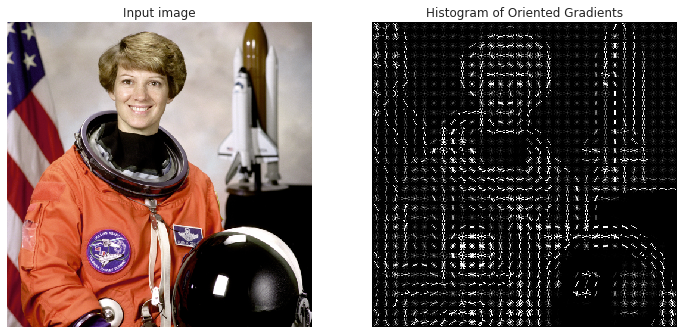
\includegraphics[width=0.4\textwidth]{IMG´s/ejemplo Hog.png}}
    \label{fig12}
  \end{figure}
  Esto lo realiza pasando la imagen original a escala de grises, luego se calcula el gradiente de la imagen, para así poder obtener la dirección y magnitud de los bordes. Después se divide la imagen en bloques, en donde cada bloque se divide en celdas, en donde cada celda tiene un histograma de orientación de gradientes. Finalmente se concatenan los histogramas de cada celda para obtener un histograma de orientación de gradientes por bloque.
  \item \textbf{Redes neuronales recurrentes}: este tipo de redes neuronales son muy útiles para el análisis de secuencias, ya que tienen la capacidad de recordar información de pasos anteriores. En la ``Figura~\ref{fig13}'' se puede ver un ejemplo de una red neuronal recurrente.
  \begin{figure}
    \caption{Ejemplo de una red neuronal recurrente.}
    \centerline{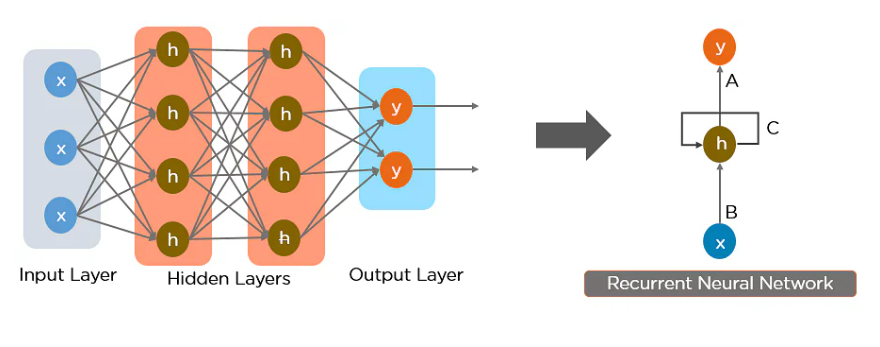
\includegraphics[width=0.5\textwidth]{IMG´s/ejemplo RNN.png}}
    \label{fig13}
  \end{figure}
  En este caso, se predefinen algunos parámetros iniciales, como el peso de la red, el número de neuronas, etc. Luego se procesan los datos de entradas y se calcula un estado interno usando los datos de entrada y datos anteriores. La parte oculta es la que se encarga de recordar información de pasos anteriores, para así poder predecir el estado futuro. Finalmente se calcula la salida usando el estado interno y los datos de entrada.
\end{itemize}

\subsection{Clasificación de polaridad}
Explora si la opinión expresada en un documento o una frase sobre una determinada característica o aspecto de un comentario es positivo, negativa o neutra. 

  Para lograr esto hay distintas estrategias, en este caso solo se hará enfoque en una específica, la cual está basada en la orientación semántica de las palabras, donde cada término que expresa opinión es anotado con un valor que representa su polaridad. En \cite{f1} menciona que este sistema, además de resolver la orientación semántica almacenada a nivel individual en adjetivos, sustantivos, verbos y adverbios; trata modificadores de la polaridad como son la negación o los intensificadores (“muy", "poco”, “bastante”, etc.…). También detecta y descarta el sentimiento reflejado en el contenido no fáctico del texto, representado, por ejemplo, mediante expresiones condicionales o subjuntivas.
Se segmenta el texto en oraciones, que a su vez se dividen para hacer la debida etiquetación, esto se ve ilustrado en la ``Figura~\ref{fig1}'', además se apoyan en diccionarios que clasifican las palabras en rangos numéricos, los cuales, mientras más tiendan a negativo, peor será el comentario y viceversa, una idea de estos diccionarios se ve representada en la ``Figura~\ref{fig2}''.
  \begin{figure}[htbp]
    \caption{Segmentación de una oración.}
    \centerline{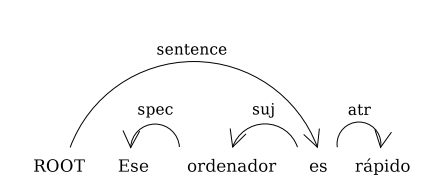
\includegraphics[width=0.45\textwidth]{IMG´s/Figura1.png}}
    \label{fig1}
  \end{figure}
  
  \begin{figure}[htbp]
    \caption{Ejemplo de un diccionarios.}
    \centerline{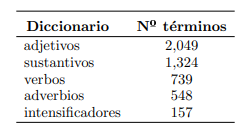
\includegraphics[width=0.4\textwidth]{IMG´s/Figura2.png}}
    \label{fig2}
  \end{figure}

\section{Conclusiones}
De forma resumida, el análisis de sentimientos es una técnica de gran importancia en el procesamiento de lenguaje natural que se utiliza para extraer información subjetiva de los textos. En este survey se presentó todo un recorrido por los distintos conceptos, casos de uso, técnicas y limitaciones en este tipo de análisis de procesamiento.
A medida que se siga globalizando el mundo y los datos se sigan acumulando de forma incremental y masiva, el análisis de sentimientos se convertirá en una herramienta que cada vez será más utilizada en la toma de decisiones, análisis de pensamiento y comportamiento humano, predicciones de eventos, tendencias, etc.
En conclusión, el análisis de sentimientos es una técnica muy valiosa para la extracción de información que no queda explícita en los textos, pero que es una área que abarca muchos campos y ofrece una gran variedad de técnicas y herramientas que dependerán del contexto y ámbito en el que se aplique.

\begin{thebibliography}{00}
  % Citas de Hansol
  \bibitem{b1} Yue, L., Chen, W., Li, X. et al. A survey of sentiment analysis in social media. Knowl Inf Syst 60, 617–663 (2019).
  \bibitem{b2} Nandwani, P., Verma, R. A review on sentiment analysis and emotion detection from text. Soc. Netw. Anal. Min. 11, 81 (2021).
  \bibitem{b3} PS, S. and Mahalakshmi, G., 2017. Emotion models: a review. International Journal of Control Theory and Applications, 10(8), pp.651-657.
  \bibitem{b4} Yaghoobian, H., Arabnia, H.R. and Rasheed, K., 2021. Sarcasm detection: A comparative study. arXiv preprint arXiv:2107.02276.
  \bibitem{b5} Gonçalves, P., Araújo, M., Benevenuto, F., and Cha, M. 2013. Comparing and Combining Sentiment Analysis Methods. In Proceedings of the First ACM Conference on Online Social Networks (pp. 27–38). Association for Computing Machinery.
  \bibitem{b6} Nadkarni, P.M., Ohno-Machado, L. and Chapman, W.W., 2011. Natural language processing: an introduction. Journal of the American Medical Informatics Association, 18(5), pp.544-551.
  \bibitem{b7} Jurafsky, D. and Martin, J.H., 2008. Speech and language processing. 2nd edn Englewood Cliffs. NJ: Prentice Hall.
  \bibitem{b8} Manning, C. and Schutze, H., 1999. Foundations of statistical natural language processing. MIT press.
  \bibitem{b9} Webster, J.J. and Kit, C., 1992. Tokenization as the initial phase in NLP. In COLING 1992 volume 4: The 14th international conference on computational linguistics.
  \bibitem{b10} Van den Bosch, A. and Buchholz, S., 2002, July. Shallow parsing on the basis of words only: A case study. In Proceedings of the 40th Annual Meeting of the Association for Computational Linguistics (pp. 433-440).
  \bibitem{b11} Hammerton, J., Osborne, M., Armstrong, S. and Daelemans, W., 2002. Introduction to the special issue on machine learning approaches to shallow parsing. Journal of machine learning research.-Cambridge, Mass., 2, pp.551-558.
  \bibitem{b12} Hashimoto, K., Xiong, C., Tsuruoka, Y. and Socher, R., 2016. A joint many-task model: Growing a neural network for multiple NLP tasks. arXiv preprint arXiv:1611.01587.
  \bibitem{b13} Schmaltz, A., Kim, Y., Rush, A., and Shieber, S. 2016. Sentence-Level Grammatical Error Identification as Sequence-to-Sequence Correction. In Proceedings of the 11th Workshop on Innovative Use of NLP for Building Educational Applications (pp. 242–251). Association for Computational Linguistics.
  \bibitem{b14} Wang, X., Liu, Y., Li, J., Miljanic, V., Zhao, S., and Khalil, H.. (2022). Towards Contextual Spelling Correction for Customization of End-to-end Speech Recognition Systems.
  \bibitem{b15} Chiu, J., and Nichols, E.. (2015). Named Entity Recognition with Bidirectional LSTM-CNNs.
  \bibitem{b16} Ma, X., and Hovy, E.. (2016). End-to-end Sequence Labeling via Bi-directional LSTM-CNNs-CRF.
  \bibitem{b17} Nadeau, D., and Sekine, S. 2007. A Survey of Named Entity Recognition and Classification. Lingvisticae Investigationes, 30.
  \bibitem{b18} Moradi, B., Ansari, E., and Zdeněkžabokrtsk´y, Z. 2019. Unsupervised Word Sense Disambiguation Using Word Embeddings. In undefined.
  \bibitem{b19} Li, X., Zhu, G., Guo, X. and Chen, W., 2015. Spatial and Temporal Word Spectrum of Social Media.
  \bibitem{b20} Iti Chaturvedi, Erik Cambria, Roy E. Welsch, and Francisco Herrera 2018. Distinguishing between facts and opinions for sentiment analysis: Survey and challenges. Information Fusion, 44, p.65-77.
  \bibitem{b21} Yadav, K., Kumar, N., Maddikunta, P.K.R. and Gadekallu, T.R., 2021. A comprehensive survey on aspect-based sentiment analysis. International Journal of Engineering Systems Modelling and Simulation, 12(4), pp.279-290.
  \bibitem{b22} Clarkson, P. and Robinson, T., 1999, September. Towards improved language model evaluation measures. In EuroSpeech.
  \bibitem{b23} Azzopardi, L., Girolami, M. and Van Risjbergen, K., 2003, July. Investigating the relationship between language model perplexity and IR precision-recall measures. In Proceedings of the 26th annual international ACM SIGIR conference on Research and development in informaion retrieval (pp. 369-370).
  \bibitem{b24} Moore, R.C. and Lewis, W., 2010, July. Intelligent selection of language model training data. In Proceedings of the ACL 2010 conference short papers (pp. 220-224).
  \bibitem{b25} Iyer, R., Ostendorf, M. and Meteer, M., 1997, December. Analyzing and predicting language model improvements. In 1997 IEEE Workshop on Automatic Speech Recognition and Understanding Proceedings (pp. 254-261). IEEE.
  \bibitem{b26} Clarkson, P. and Robinson, T., 2001. Improved language modelling through better language model evaluation measures. Computer Speech \& Language, 15(1), pp.39-53.
  % Citas de Randall
  \bibitem{r1} El-Din, D.M., 2016. Enhancement bag-of-words model for solving the challenges of sentiment analysis. International Journal of Advanced Computer Science and Applications, 7(1).
  \bibitem{r2} López, G.J. and Ruiz, I.M., 2016. Character and word baselines systems for irony detection in Spanish short texts. Procesamiento del Lenguaje Natural, 56, pp.41-48.
  \bibitem{r3} De Gemmis, M., Lops, P., Semeraro, G. and Basile, P., 2008, October. Integrating tags in a semantic content-based recommender. In Proceedings of the 2008 ACM conference on Recommender systems (pp. 163-170).
  \bibitem{r4} Mukherjee, S. and Bala, P.K., 2017. Sarcasm detection in microblogs using Naïve Bayes and fuzzy clustering. Technology in Society, 48, pp.19-27.
  \bibitem{r5} Vanzo, A., Croce, D. and Basili, R., 2014, August. A context-based model for sentiment analysis in twitter. In Proceedings of coling 2014, the 25th international conference on computational linguistics: Technical papers (pp. 2345-2354).
  \bibitem{r6} Thorne, J., A Convolution Kernel for Sentiment Analysis using Word-Embeddings.
  \bibitem{r7} Federico, P., Heimerl, F., Koch, S. and Miksch, S., 2016. A survey on visual approaches for analyzing scientific literature and patents. IEEE transactions on visualization and computer graphics, 23(9), pp.2179-2198.
  \bibitem{r8} Asghar, M.Z., Ahmad, S., Marwat, A. and Kundi, F.M., 2015. Sentiment analysis on youtube: A brief survey. arXiv preprint arXiv:1511.09142.
  \bibitem{r9} Cunha, A.A.L., Costa, M.C. and Pacheco, M.A.C., 2019. Sentiment analysis of youtube video comments using deep neural networks. In Artificial Intelligence and Soft Computing: 18th International Conference, ICAISC 2019, Zakopane, Poland, June 16–20, 2019, Proceedings, Part I 18 (pp. 561-570). Springer International Publishing.
  \bibitem{r19} Y. Tsuboi, A. Jatowt and K. Tanaka, "Product Purchase Prediction Based on Time Series Data Analysis in Social Media," 2015 IEEE/WIC/ACM International Conference on Web Intelligence and Intelligent Agent Technology (WI-IAT), Singapore, 2015, pp. 219-224, doi: 10.1109/WI-IAT.2015.170.
  \bibitem{r18} Joyojeet Pal, and A'Ndre Gonawela 2017. Studying political communication on Twitter: the case for small data. Current Opinion in Behavioral Sciences, 18, p.97-102.
  \bibitem{r17} V. S. Pagolu, K. N. Reddy, G. Panda and B. Majhi, "Sentiment analysis of Twitter data for predicting stock market movements," 2016 International Conference on Signal Processing, Communication, Power and Embedded System (SCOPES), Paralakhemundi, India, 2016, pp. 1345-1350, doi: 10.1109/SCOPES.2016.7955659.
  \bibitem{r16} Klaifer Garcia, and Lilian Berton 2021. Topic detection and sentiment analysis in Twitter content related to COVID-19 from Brazil and the USA. Applied Soft Computing, 101, p.107057.
  \bibitem{r15} Kerstin Denecke, and Yihan Deng 2015. Sentiment analysis in medical settings: New opportunities and challenges. Artificial Intelligence in Medicine, 64(1), p.17-27.
  \bibitem{r14} Misirana, M. ., Tan, S. E. ., Augustus Saw, P. H. ., Mohd Subri, N. A. ., Ahmad Darus, N. S. ., Md Yusof, Z. ., \& Ahmad, N. . (2021). Early Detection Method for Money Fraudulent Activities on E-commerce Platform via Sentiment Analysis. Journal of Entrepreneurship and Business, 9(2), 121–142.
  % Citas de Fredd
  \bibitem{f1} Vilares, D., Alonso, M.A. and Gómez-Rodríguez, C., 2013. Clasificación de polaridad en textos con opiniones en espanol mediante análisis sintáctico de dependencias. Procesamiento del lenguaje natural, 50, pp.13-20.
  \bibitem{f2} Wankhade, M., Rao, A.C.S. \& Kulkarni, C. A survey on sentiment analysis methods, applications, and challenges. Artif Intell Rev 55, 5731–5780 (2022).
  \bibitem{f3} Tong Xue, Surjya Ghosh, Gangyi Ding, Abdallah El Ali, and Pablo Cesar. 2020. Designing Real-time, Continuous Emotion Annotation Techniques for 360° VR Videos. In Extended Abstracts of the 2020 CHI Conference on Human Factors in Computing Systems (CHI EA '20). Association for Computing Machinery, New York, NY, USA, 1–9.
  \bibitem{f4} L. Canales, W. Daelemans, E. Boldrini and P. Martínez-Barco, \"EmoLabel: Semi-Automatic Methodology for Emotion Annotation of Social Media Text,\" in IEEE Transactions on Affective Computing, vol. 13, no. 2, pp. 579-591.
  \bibitem{f5} Roberts, K., Roach, M.A., Johnson, J., Guthrie, J. and Harabagiu, S.M., 2012, May. EmpaTweet: Annotating and Detecting Emotions on Twitter. In Lrec (Vol. 12, No. 12, pp. 3806-3813).
  \bibitem{f6} Frantova, E. and Bergler, S., 2009. Automatic emotion annotation of dream diaries. In Proceedings of the analyzing social media to represent collective knowledge workshop at K-CAP 2009, The fifth international conference on knowledge capture.
  \bibitem{f7} Maite Taboada, Julian Brooke, Milan Tofiloski, Kimberly Voll, Manfred Stede; Lexicon-Based Methods for Sentiment Analysis. Computational Linguistics 2011; 37 (2): 267–307.
  \bibitem{f8} Dumais, S.T., 2004. Latent semantic analysis. Annu. Rev. Inf. Sci. Technol., 38(1), pp.188-230.
  \bibitem{f9} Thomas K Landauer, Peter W. Foltz, and Darrell Laham 1998. An introduction to latent semantic analysis. Discourse Processes, 25(2-3), p.259-284.
  \bibitem{f10} Soboroff, I., Nicholas, C., Kukla, J., and Ebert, D. 1998. Visualizing Document Authorship Using N-grams and Latent Semantic Indexing
  \bibitem{f11} Rosa, R.L., Rodríguez, D.Z., Schwartz, G.M., de Campos Ribeiro, I. and Bressan, G., 2016, January. Monitoring system for potential users with depression using sentiment analysis. In 2016 IEEE International Conference on Consumer Electronics (ICCE) (pp. 381-382). Ieee.
  \bibitem{f12} B. S. Atote, T. S. Saini, M. Bedekar and S. Zahoor, \"Inferring emotional state of a user by user profiling,\" 2016 2nd International Conference on Contemporary Computing and Informatics (IC3I), Greater Noida, India, 2016, pp. 530-535.
  \bibitem{f13} K. Patel et al., "Facial Sentiment Analysis Using AI Techniques: State-of-the-Art, Taxonomies, and Challenges," in IEEE Access, vol. 8, pp. 90495-90519, 2020
  \bibitem{f14} Chi-Chun Lee, Emily Mower, Carlos Busso, Sungbok Lee, and Shrikanth Narayanan 2011. Emotion recognition using a hierarchical binary decision tree approach. Speech Communication, 53(9), p.1162-1171.
  
  

\end{thebibliography}


\end{document}
